%% CS854 RadixVM Presentation
%% Winter 2016

%%% BEGIN PREAMBLE
\documentclass[aspectratio=169]{beamer}
\usepackage{hyperref}
\usepackage{color}

%% Smart underlining -- from cdi-macros.tex
\def\ul#1{$\underline{\smash{\hbox{#1}}}$}

% TikZ packages (for graphs)
%\usepackage{tkz-graph}
%\usepackage{tkz-berge}
%\usetikzlibrary{snakes}

%% Shortcuts

\newcommand{\bi}{\begin{itemize}}
\newcommand{\ei}{\end{itemize}}

\newcommand{\bn}{\begin{enumerate}}
\newcommand{\en}{\end{enumerate}}

\newcommand{\bd}{\begin{description}}
\newcommand{\ed}{\end{description}}

\mode<presentation>
{
  \usetheme{Madrid}
  \usecolortheme{beaver}
}
\usepackage[english]{babel}

\usepackage{times}
\usepackage[T1]{fontenc}
% Note that the encoding and the font should match. If T1 does not
% look nice, try deleting the line with the fontenc.

\title{RadixVM}
\subtitle{Scalable address spaces for multithreaded applications}

\author[Presented by Simon Pratt]{Austin T. Clements,\\M. Frans Kaashoek,\\Nickolai Zeldovich\\
  \vspace{2em}Presented by Simon Pratt}

\date{February 12, 2016}


%%% BEGIN DOCUMENT
\begin{document}

\frame[plain]{\titlepage}

\newpage

\begin{frame}{Abstract}
  RadixVM is a virtual memory (VM) design that attempts to increase multithreaded scalability by:
  \bi
\item Storing VM information in a radix tree
\item Counting references to memory addresses
\item Reducing inter-core virtual address invalidation\\(remote TLB shootdown)
  \ei
\end{frame}

\section{Background}

\begin{frame}{Background: Virtual Memory}
  \begin{columns}[T]
    \begin{column}{0.3\textwidth}
      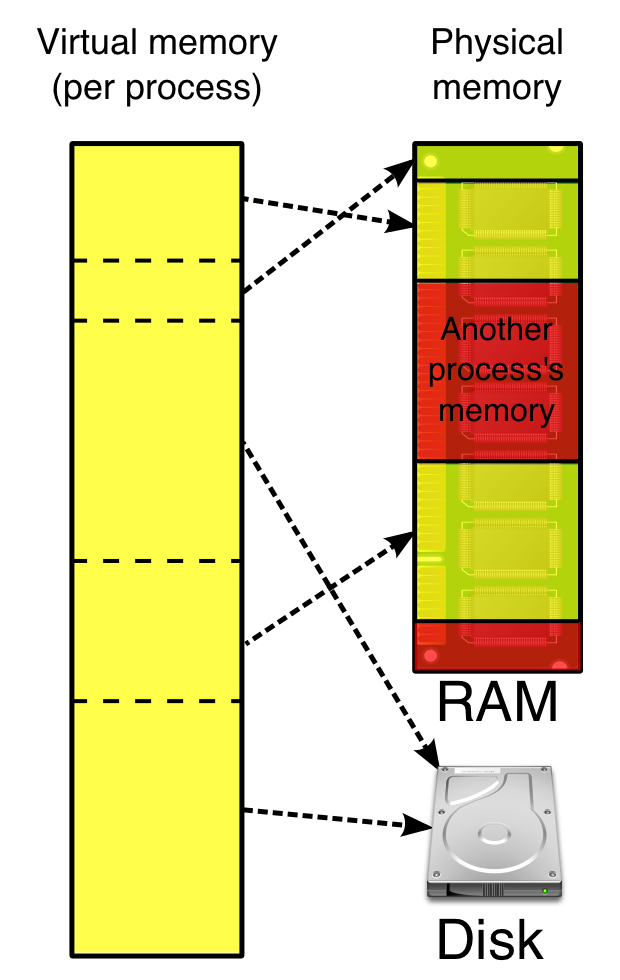
\includegraphics[scale=0.2]{./figures/Virtual_memory.png}
    \end{column}
    \begin{column}{0.7\textwidth}
      \bi
    \item Maps a contiguous virtual address space to:
      \bi
    \item physical memory (frames)
    \item disk (swap)
      \ei
      \ei
    \end{column}
  \end{columns}
\end{frame}

\begin{frame}{Background: \texttt{malloc} and \texttt{mmap}}
  \begin{columns}[T]
    \begin{column}{0.2\textwidth}
      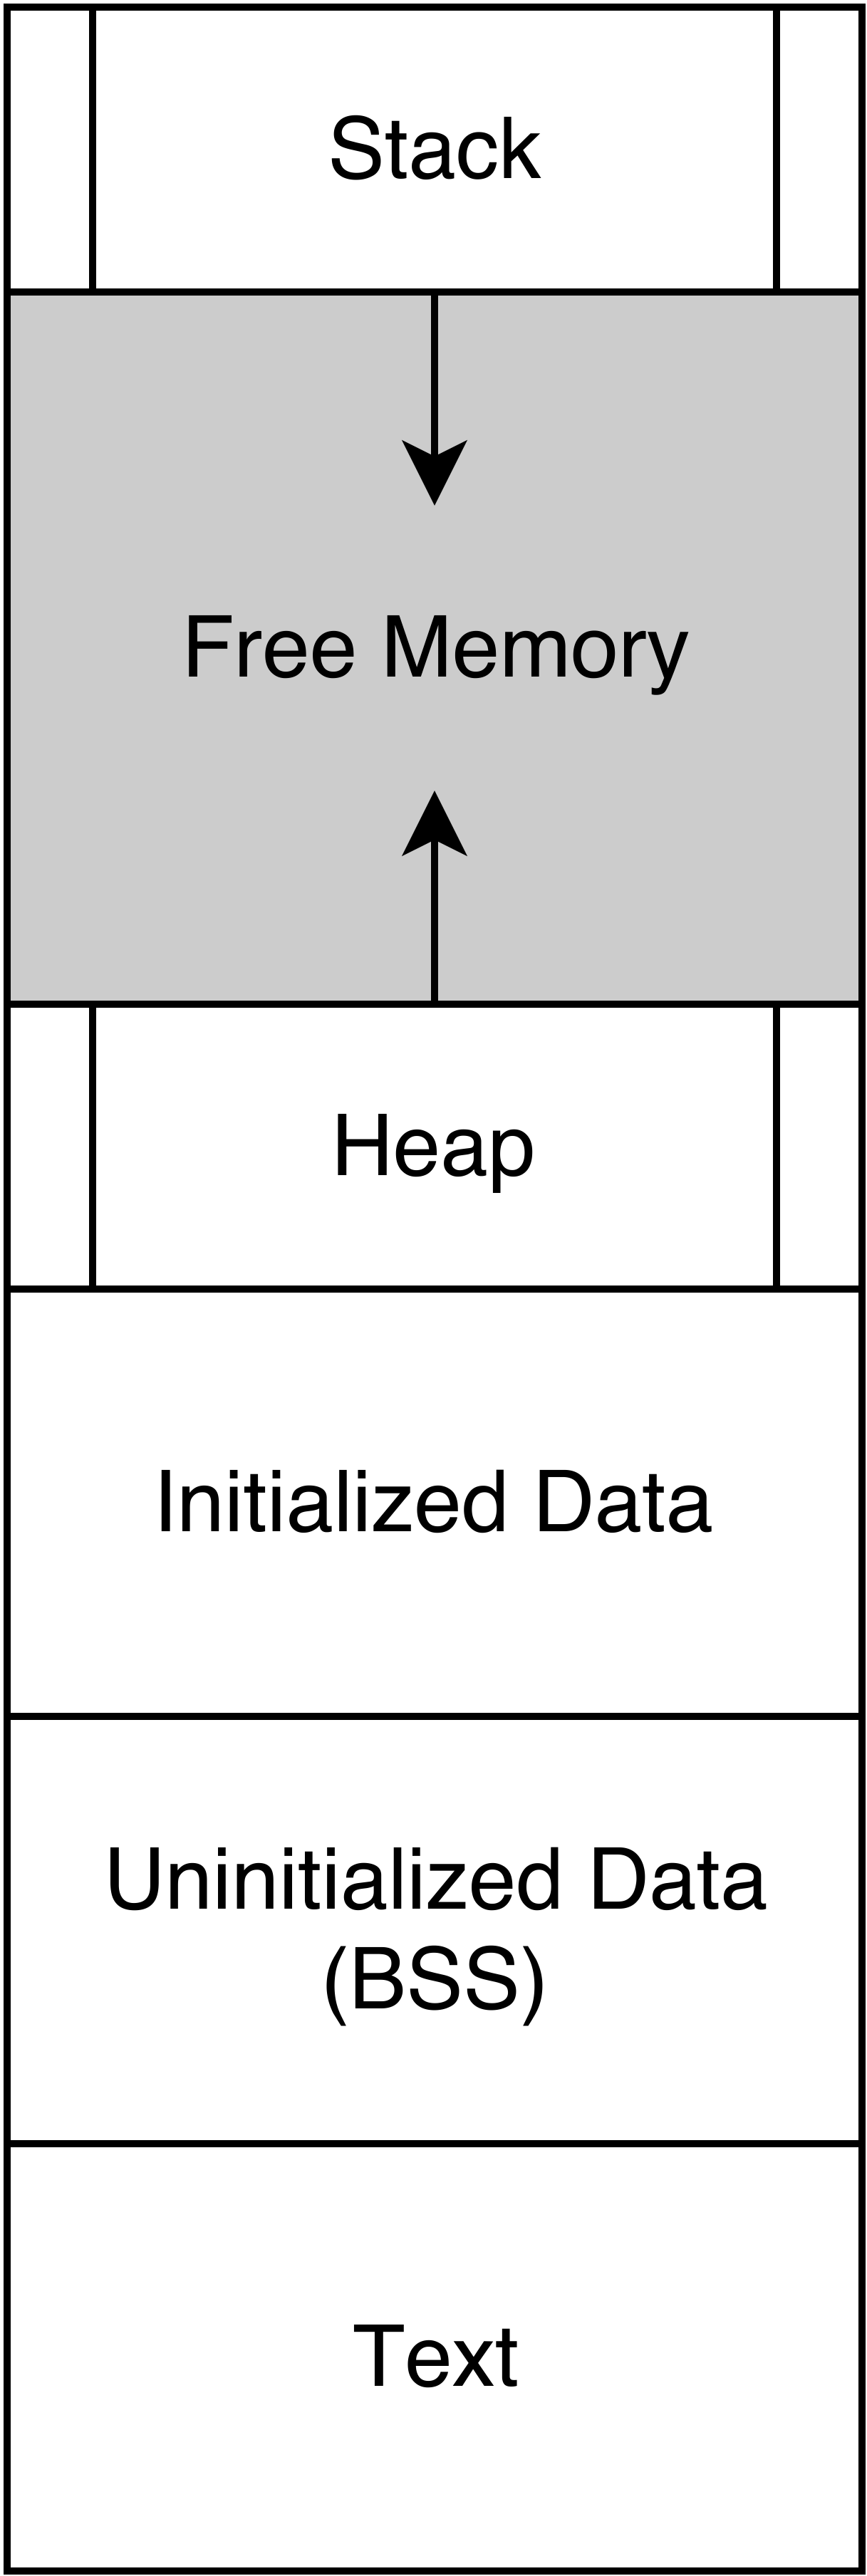
\includegraphics[scale=0.05]{./figures/Address_space.png}
    \end{column}
    \begin{column}{0.8\textwidth}
      \bi
    \item \texttt{malloc} and \texttt{free}
      \bi
    \item User-level library function
    \item Allocates/frees space in virtual memory
    \item Often implemented using \texttt{mmap} and \texttt{munmap}
      \ei
    \item \texttt{mmap} and \texttt{munmap}
      \bi
    \item System calls
    \item Actually allocates/frees space in virtual memory
      \ei
      \ei
    \end{column}
  \end{columns}
\end{frame}

\begin{frame}{Background: Linux Virtual Memory}
  \begin{center}
    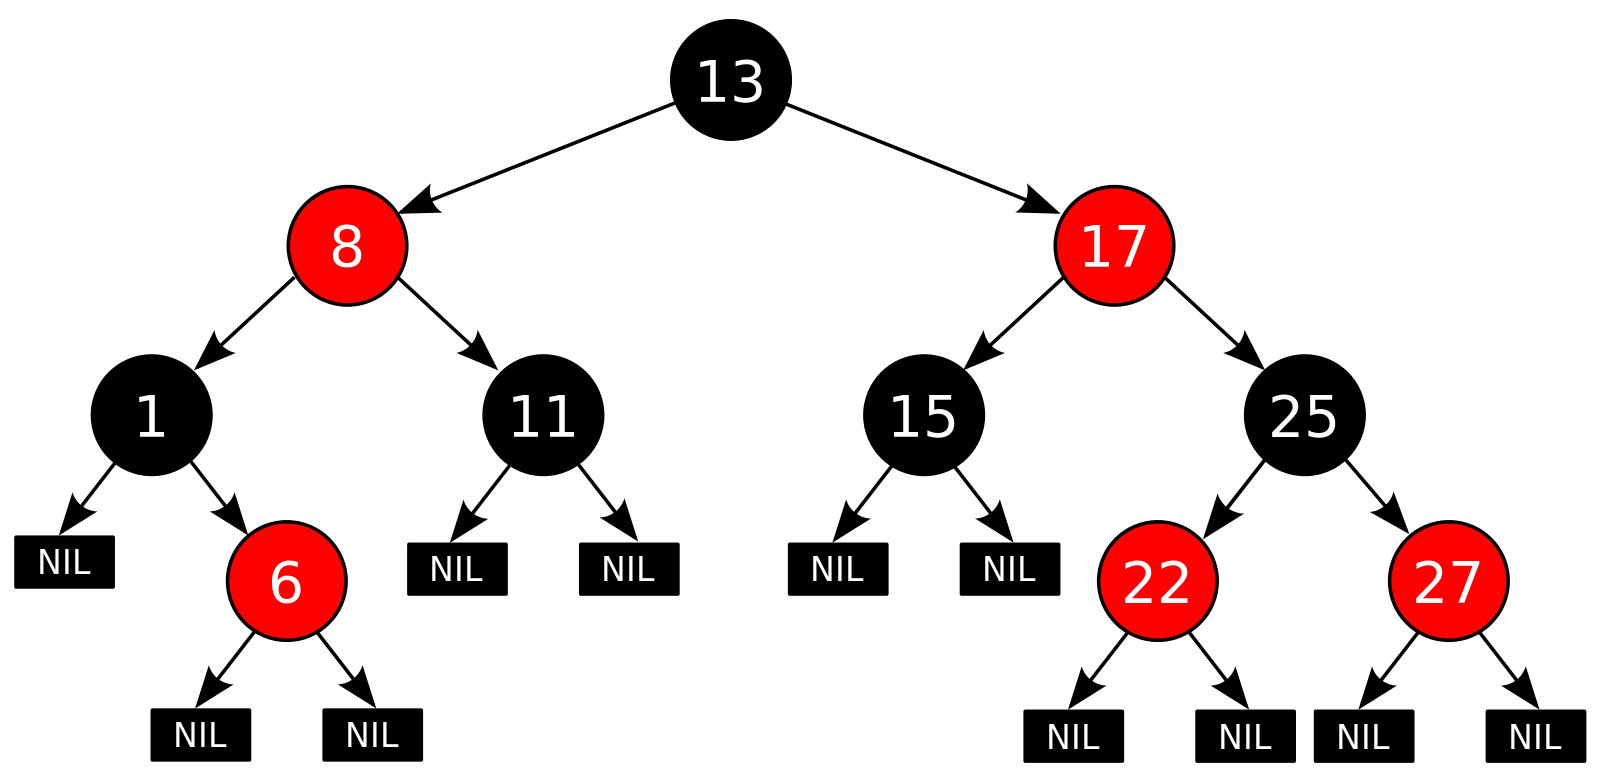
\includegraphics[scale=0.2]{./figures/Red-black_tree.png}
    \bi
    \item Red-black tree
    \item Allows the kernel to search for memory area covering a virtual address
      \pause
    \item \color{red}{Problem: A single lock per address space!}
    \ei
  \end{center}
\end{frame}

\section{Design}

\begin{frame}{Design: High-level}
  RadixVM has 3 parts:
  \begin{center}
    \bi
  \item Refcache
  \item Radix-tree-like data structure
  \item Targeted TLB shootdowns
    \ei
  \end{center}
\end{frame}

\begin{frame}{Background: ABA Problem}
  \begin{center}
    TODO
    \bi
  \item Major issue in lock-free data structures
  \item Roughly:
    \bi
  \item Process $P_1$ reads value $A$ in memory location
  \item Process $P_2$ changes the value to $B$
  \item Process $P_2$ changes the value back to $A$
  \item Process $P_1$ reads value $A$ in memory location again, and assumes nothing has changed
    \ei
    \ei
  \end{center}
\end{frame}

\begin{frame}{Design: Refcache}
  \begin{columns}[T]
    \begin{column}{0.2\textwidth}
      TODO
    \end{column}
    \begin{column}{0.8\textwidth}
      \bi
    \item Counts references to memory locations
    \item Divides time into epochs
    \item Frees memory when a memory location is unreferenced for an entire epoch
    \item Solves the ABA problem
      \ei
    \end{column}
  \end{columns}
\end{frame}

\begin{frame}{Background: Radix Tree}
  \begin{center}
    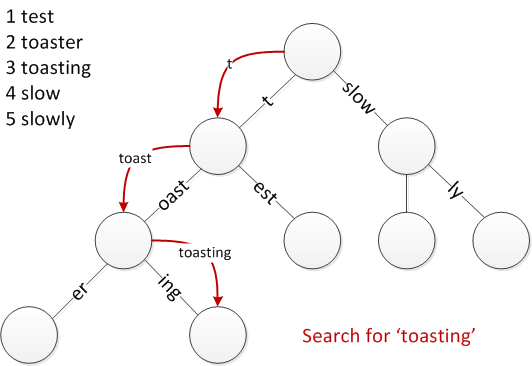
\includegraphics[scale=0.5]{./figures/Patricia_trie.png}
    \bi
  \item A.K.A. prefix tree
  \item Edges labeled
  \item Concatenation of edge labels along root$\rightarrow$node path gives a string
  \item In OSes, usually strings of bits
    \ei
  \end{center}
\end{frame}

\begin{frame}{Design: RadixVM Data Structure}
  \begin{columns}[T]
    \begin{column}{0.2\textwidth}
      TODO
    \end{column}
    \begin{column}{0.8\textwidth}
      \bi
    \item Similar to a radix-tree
    \item Fixed-height
    \item Each level indexed by up to 9 bits
      \ei
    \end{column}
  \end{columns}
\end{frame}

\begin{frame}{Background: Remote TLB Shootdowns}
  \begin{columns}[T]
    \begin{column}{0.2\textwidth}
      TODO
    \end{column}
    \begin{column}{0.8\textwidth}
      When a shared memory location is unmapped:
      \bi
    \item The TLB for every core is flushed
    \item \color{red}{This is expensive!}
      \ei
    \end{column}
  \end{columns}
\end{frame}

\begin{frame}{Design: Targeted TLB Shootdowns}
  \begin{columns}[T]
    \begin{column}{0.2\textwidth}
      TODO
    \end{column}
    \begin{column}{0.8\textwidth}
      \bi
    \item Store metadata on which cores may have address in TLB
    \item Only flush TLBs on cores which may share that memory
      \ei
    \end{column}
  \end{columns}
\end{frame}

\begin{frame}{Design: Do we need all 3 pieces?}
  \begin{columns}[T]
    \begin{column}{0.2\textwidth}
      TODO
    \end{column}
    \begin{column}{0.8\textwidth}
      \bi
    \item TODO
      \ei
    \end{column}
  \end{columns}
\end{frame}

\section{Performance}

\begin{frame}{Implementation}
  \begin{center}
    \bi
  \item Implemented on xv6
    \bi
  \item Academic OS
  \item Based on v6 Unix
  \item Rewritten in ANSI C for x86
  \item \url{https://pdos.csail.mit.edu/6.828/2014/xv6.html}
    \ei
    \ei
  \end{center}
\end{frame}

\begin{frame}{Application: Metis}
  \begin{columns}[T]
    \begin{column}{0.2\textwidth}
      TODO
    \end{column}
    \begin{column}{0.8\textwidth}
      \bi
    \item MapReduce Library
    \item Single-server
    \item Multithreaded
    \item Stresses concurrent \texttt{mmap}s and \texttt{pagefault}s, but not concurrent \texttt{munmap}s
    \item Compiles on xv6 and linux
      \ei
    \end{column}
  \end{columns}
\end{frame}

\begin{frame}{Microbenchmark: Local}
  \begin{columns}[T]
    \begin{column}{0.2\textwidth}
      TODO
    \end{column}
    \begin{column}{0.8\textwidth}
      \bi
    \item \texttt{mmap} a private 4KB region in shared address space
    \item Write to every page in region
    \item \texttt{munmap} region
      \ei
    \end{column}
  \end{columns}
\end{frame}

\begin{frame}{Microbenchmark: Pipeline}
  \begin{columns}[T]
    \begin{column}{0.2\textwidth}
      TODO
    \end{column}
    \begin{column}{0.8\textwidth}
      \bi
    \item Each thread \texttt{mmap} a region
    \item Write to every page in region
    \item Pass region to next thread
    \item Write to every page in passed region
    \item \texttt{munmap} region
      \ei
    \end{column}
  \end{columns}
\end{frame}

\begin{frame}{Microbenchmark: Global}
  \begin{columns}[T]
    \begin{column}{0.2\textwidth}
      TODO
    \end{column}
    \begin{column}{0.8\textwidth}
      \bi
    \item Each thread \texttt{mmap} a 64KB region within a large region of memory
    \item All threads access all pages in random order
      \ei
    \end{column}
  \end{columns}
\end{frame}

\begin{frame}{Memory Overhead}
  \begin{center}
    \begin{tabular}{ l | c | c c | c }
              &        & \multicolumn{2}{c|}{Linux} & Radix tree \\
              & RSS    & VMA tree & Page table      & (rel. to Linux) \\
      \hline
      Firefox & 352 MB & 117 KB   & 1.5 MB          & 3.9 MB (2.4$\times$) \\
      Chrome  & 152 MB & 124 KB   & 1.1 MB          & 2.4 MB (2.0$\times$) \\
      Apache  & 16 MB  & 44 KB    & 368 KB          & 616 KB (1.5$\times$) \\
      MySQL   & 84 MB  & 18 KB    & 348 KB          & 980 KB (2.7$\times$) \\
    \end{tabular}
    \vspace{1em}
    \bi
  \item RSS
    \bi
  \item Resident Set Size
  \item physical memory used by a process
    \ei
  \item VMA
    \bi
  \item Virtual Memory Areas
  \item stored in a red-black tree in Linux
    \ei
    \ei
  \end{center}
\end{frame}

\begin{frame}{Summary}
  \begin{columns}[T]
    \begin{column}{0.2\textwidth}
      TODO
    \end{column}
    \begin{column}{0.8\textwidth}
      \bi
    \item TODO
      \ei
    \end{column}
  \end{columns}
\end{frame}

% Structuring a talk is a difficult task and the following structure
% may not be suitable. Here are some rules that apply for this
% solution: 

% - Exactly two or three sections (other than the summary).
% - At *most* three subsections per section.
% - Talk about 30s to 2min per frame. So there should be between about
%   15 and 30 frames, all told.

% - A conference audience is likely to know very little of what you
%   are going to talk about. So *simplify*!
% - In a 20min talk, getting the main ideas across is hard
%   enough. Leave out details, even if it means being less precise than
%   you think necessary.
% - If you omit details that are vital to the proof/implementation,
%   just say so once. Everybody will be happy with that.

\begin{frame}[noframenumbering]{References}
  \bi
\item Clements, Austin T., M. Frans Kaashoek, and Nickolai Zeldovich. "RadixVM: Scalable address spaces for multithreaded applications." In \emph{Proceedings of the 8th ACM European Conference on Computer Systems}, pp. 211-224. ACM, 2013.
  \item Revised version: \url{https://pdos.csail.mit.edu/papers/radixvm:eurosys13-2014-08-05.pdf}
\item Linux VM info from:\\ \url{http://duartes.org/gustavo/blog/post/how-the-kernel-manages-your-memory/}
  \ei
\end{frame}

\begin{frame}[noframenumbering]{Attribution}
  \bi
\item Virtual memory diagram by Ehamberg (Own work) [CC BY-SA 3.0 (\url{http://creativecommons.org/licenses/by-sa/3.0}) or GFDL (\url{http://www.gnu.org/copyleft/fdl.html})], via Wikimedia Commons
\item Address space diagram by Majenko (Own work) [CC BY-SA 4.0 (\url{http://creativecommons.org/licenses/by-sa/4.0})], via Wikimedia Commons
\item Patricia trie diagram by Saffles (Microsoft Visio) [GFDL (\url{http://www.gnu.org/copyleft/fdl.html}) or CC BY-SA 3.0 (\url{http://creativecommons.org/licenses/by-sa/3.0})], via Wikimedia Commons
  \ei
\end{frame}

\end{document}



